\documentclass[11pt,a4paper]{article}
\usepackage[T1]{fontenc}
\renewcommand{\rmdefault}{ptm}
\renewcommand{\ttdefault}{pcr}
\renewcommand{\sfdefault}{phv}
\usepackage{amsmath,amssymb,amsthm,graphicx,booktabs}
\usepackage[cmintegrals]{newtxmath}
\usepackage[margin=24mm]{geometry}
% Load in the document preamble. Figures are native TikZ/PGFPlots.
% No external graphics, conversion programs, or shell escape are required.
\usepackage{tikz,pgfplots}
\pgfplotsset{compat=1.18}
\usetikzlibrary{arrows.meta,calc}
\definecolor{jscNavy}{HTML}{08457E}
\definecolor{jscTeal}{HTML}{087F78}
\definecolor{jscBlue}{HTML}{237BC1}
\definecolor{jscAmber}{HTML}{B87708}
\definecolor{jscGrey}{HTML}{86A2B6}
\definecolor{jscPale}{HTML}{E9EFF3}
\definecolor{jscBand}{HTML}{CFE5E4}
\definecolor{jscDark}{HTML}{173B55}
\definecolor{jscRed}{HTML}{A6423A}
\definecolor{jscLight}{HTML}{CBD6DE}
\definecolor{jscUnresolved}{HTML}{AB403B}
\definecolor{jscGrid}{HTML}{DCE4E9}
\definecolor{jscRadio}{HTML}{0072B2}
\definecolor{jscServer}{HTML}{D55E00}
\definecolor{jscBoth}{HTML}{009E73}
\newcommand{\jscfont}[1]{\rmfamily\fontsize{#1}{\dimexpr#1pt+2pt\relax}\selectfont}
\providecommand{\jscDataPath}{figures/tikz/data}
\pgfplotsset{jsc axis/.style={
    scale only axis,axis lines=left,axis line style={-,line width=.7pt},
    tick align=outside,tick style={line width=.6pt},
    tick label style={font=\jscfont{7}},
    label style={font=\jscfont{8}},
    title style={font=\jscfont{8}},
    scaled ticks=false,
    /pgf/number format/1000 sep={\,},
    clip mode=individual,
  }}

\usepackage{flafter}
\usepackage[hidelinks]{hyperref}
\hypersetup{pdftitle={Service Certification for Agentic Wireless Networks: Extended Experiments and Code},pdfauthor={Saeed Razavikia and Carlo Fischione}}
\newcommand{\T}{\mathsf{T}}
\newcommand{\range}{\operatorname{range}}
\newcommand{\norm}[1]{\left\lVert#1\right\rVert}
\newenvironment{IEEEproof}{\begin{proof}}{\end{proof}}
\newtheorem{theorem}{Theorem}
\title{Service Certification for Agentic Wireless Networks:\\Extended Experiments and Code}
\author{Saeed Razavikia \and Carlo Fischione}
\date{}
\setlength{\emergencystretch}{2em}
\begin{document}
\maketitle
This research archive accompanies \emph{Service Certification for Agentic Wireless Networks: Principles and Fundamental Limits}. We collect the complete experimental description from the supplied supplementary source, including additional numerical comparisons, figure data, and limitations. We retain each study's own population, comparator, and resource accounting.

\paragraph{Available material.} The package supplies plotting scripts, summary data, editable figures, and protocol descriptions. The original simulation/controller drivers, complete trial records, and research directories cited in the source manuscript were not supplied. Accordingly, the scripts regenerate available figures; they do not rerun those experiments. Unmodified source fragments remain in \texttt{docs/source/}, and \texttt{docs/provenance.md} maps their contents. Statements about historical numerical outcomes below report the supplied manuscript's results, without asserting a new experimental replay.

\section*{Definitions for this standalone protocol}
For the nine-pair wireless instance, $R_i$, $f_j$, and $t_j$ denote radio rate, processor rate, and transport delay. The supplied manuscript sets $R=(20.574,51.891,100.556)$ Mbit/s, $f=(1,2,3)$ GHz, and $t=(0.8,1.2,1.8)$ ms. Tasks contain 80 kbit and require eight million processor cycles. With radio and server corrections $r_i,w_j$ in ms, we use
\begin{equation}
\begin{aligned}
D_{ij}(\theta)&=d^0_{ij}+r_i+w_j, &d^0_{ij}&=80/R_i+8/f_j+t_j,\\
D_i^{\rm rad}(\theta)&=80/R_i+r_i.
\end{aligned}
\label{eq:wireless-delay}
\end{equation}
Charges satisfy $p_{ij}=p_i^{\rm rad}+p_j^{\rm srv}$, with $p^{\rm rad}=(1,2,3.6)$ and $p^{\rm srv}=(0.6,1.4,2.8)$. For goal parameters $(\alpha_g,T_g,T_g^{\rm rad})$, the service decision is
\begin{equation}
\begin{aligned}
\min_{i,j}\quad &p_{ij}+\alpha_g D_{ij}(\theta)\\
\text{subject to}\quad &D_{ij}(\theta)\leq T_g,\\
&D_i^{\rm rad}(\theta)\leq T_g^{\rm rad}\quad\text{when requested}.
\end{aligned}
\label{eq:wireless-instance}
\end{equation}
The acquisition studies set $\alpha_g=0$. Symbol $\Phi$ denotes the standard normal cdf and $z_p=\Phi^{-1}(p)$. The following reference restates the scalar frontier used by the protocol; its proof remains in the paper and theoretical supplement.
\begin{theorem}[Exact scalar completion reference]
\label{thm:scalar-deadline}
For centered Gaussian probe means $a_e\vartheta$, let $q_e=a_e^2/\sigma_e^2$ and let $A_{\max}$ be the greatest total precision available from history and a legal integer acquisition design. For $A_{\max}>0$ and $0<\delta<1/2$, the attainable correct-completion probability at $\vartheta\ne0$ is
$$\Phi\!\left(|\vartheta|\sqrt{A_{\max}}-z_{1-\delta}\right).$$
A maximum-precision fixed design and its two-threshold endpoint rule attain this value. Completion $1-\eta>\delta$ is possible exactly when $|\vartheta|\sqrt{A_{\max}}\geq z_{1-\delta}+z_{1-\eta}$.
\end{theorem}
At zero precision, operational policies abstain; the randomized reference can attain correct completion $\delta$ by assigning probability $\delta$ to each answer.

\section{Experimental Protocols and Matched Comparisons}
\label{app:experiments}
Every comparison retains its own population, verifier, and denominator. Costs include all attempts and acquired reports; additional costs exclude sunk history, and modeled durations exclude computation. The availability statement above applies to the upstream records named in the original source.

\subsection{Wireless Model and Allocation}
\label{app:wireless-parameters}
The nine-pair fixture uses evaluation-only correction means
$$
\begin{aligned}
(r_1,r_2,r_3)&=(2.409418,1.208761,.751280),\\
(w_1,w_2,w_3)&=(6.061585,2.113124,.935895).
\end{aligned}
$$
in milliseconds. Rates use bandwidths $(10,15,20)$ MHz and SNRs $(5,10,15)$ dB. Aggregate and radio-counter directions are $a_{ij}=\mathbf e_i+\mathbf e_{3+j}$ and $\mathbf e_i$; response coefficients follow \eqref{eq:wireless-delay}--\eqref{eq:wireless-instance}. Background radio/server means are $80/R_i,5/f_j$, and tagged processor service is $8/f_j$. Workload caps $\overline w_k$ equal seven background means. Reports average $m_{\rm coh}=64$ independent finite-FCFS-population draws, with proxy
$$\sigma_e^2=(4m_{\rm coh})^{-1}\sum_k a_{e,k}^2\overline w_k^2.$$
This independence concerns synthetic diagnostics, not production packets. Aggregate costs/durations are $1+.35p_{ij}$ and $1+d_{ij}^0/20$; the R1 counter uses $12/2$ units. The window is 20000, caps are $\bar n_e=h_e+\lfloor20000/\ell_e\rfloor$, and no monetary cap binds separately.

\label{app:restored-comparisons}
\emph{Legacy scope.} Missing runners, seeds, paired outcomes, and bootstrap records prevent reproducing the earlier stage/wireless comparisons. Adverse cases include: scalar quotas cost 14.79 versus residual's 15.83 at 12.6 ms; loose-goal restart optimizer gaps exceed 90\%; adding a common completion safeguard reverses residual/maximin stage costs from $136.09/198.25$ to $273.63/263.25$ on 32 seeds. 

\label{app:allocation-replication}
\emph{Published-rule adaptations.} Printed G-ACOL~\cite{lindner2022} measures the most uncertain remaining configuration. Authors-code commit \texttt{33fc4d2} instead selects that target $b_u$ and maximizes its one-report variance reduction,
$$\frac{(b_u^{\T}Va_e)^2}{\sigma_e^2+a_e^{\T}Va_e},\qquad V=(M+.1I)^{-1},$$
where $M$ is accumulated weighted information. Neither rule normalizes by price; regularization affects allocation only. We adapt noise, history, stage access, batching, and the common v10 \texttt{JointVerifier}, without transferring published guarantees.

The frozen comparison uses 64 paired sequences (seeds 57000000--57000063), goals $24\to12.6\to9.5\to24$ ms, $\epsilon=\delta=.05$, and retained initial counts
$$(1024,1024,1024,1024,0,0,1024,0,0,0)$$
in saved probe order. All retain the original window/caps. Batches contain at most eight reports; residual replans within 512 with inflation 1.1. All verify after batches/phase entry; greedy phase endings add checks without observations. Intervals use 10000 complete-sequence paired bootstraps (seed 57009999).

\begin{table}[t]
\centering\small
\caption{Frozen 64-sequence allocation comparison. Every rule returns all 256 decisions correctly. Savings use each comparator's mean sequence cost; intervals are paired descriptive 95\% bootstrap intervals.}
\label{tab:allocation-replication-cost}
\label{tab:allocation-replication-savings}
\setlength{\tabcolsep}{3pt}
\begin{tabular}{@{}lrr@{}}
\toprule
Rule & Mean cost & Saving [95\% interval]\\
\midrule
Residual &2675.92&---\\
Code lookahead &2869.31&6.74\% [6.43,7.05]\%\\
Maximum variance &2881.81&7.14\% [6.83,7.47]\%\\
\bottomrule
\end{tabular}
\end{table}
Lookahead is cheaper at 12.6 ms ($9.625/9.97625$), although residual costs less over every complete sequence. No method uses a stage probe; all loose and 50/64 intermediate goals need no reports. Controller times $.124/.225/.218$ s include unequal checks and simulation. An unchanged-code check correctly returns arm 8 on eight compatible nine-arm instances (mean 290 reports), without a residual comparator. The original source identifies a separate evidence record set for these checks; it was not supplied. These checks establish neither superiority over unchanged G-ACOL nor Fast Beam Alignment; maximin uses separate tapes.

\subsection{Stopping, Calibration, and Continuation Selection}
\label{app:execution-saving}
\emph{Fixed reserve.} The archived Gaussian comparison shares preparation, reserve, confidence, and potential reports across 120 paired attempts: 45 certify initially, 44 after the pilot, 14 during completion, and 17 remain unresolved with infeasible completion designs. For full-quota, block, proportional, and goal-directed execution, the respective mean costs are $4567.93$, $1194.59$, $1023.80$, and $1022.73$. The corresponding 14-trial means are $32654.50$, $3740.21$, $2276.29$, and $2267.14$. Goal-directed savings are therefore 77.6\% overall, 93.1\% conditionally, and only .10\% against proportional stopping. A separate deterministic 93.5\% illustration is not a stochastic estimate. Original raw execution records are missing.

The separate calibration comparison is described only by reference to an unavailable earlier supplement; its population and risk grid are not pooled here.

\label{app:controller-diagnostics}
\emph{Continuation selection.} Two separate 40-decision studies retain the same resources and mixture verifier ($V_0=10I$), using four cases, five seeds, and risks $.05,.01$. The selector combines directional/balanced/single-probe bases, four discovery reports/probe, at most 100 design iterations, and 512 simulated futures/candidate. Clopper--Pearson/transport allowances are $.01$ each. The declared holdout replaces 18 quota candidates by six full-quota candidates; the complete checkpoint and tie records were not supplied.

Initial baseline/selector correct counts are $40/32$ at costs $3396.68/3534.15$; holdout counts are $40/37$ at $2881.20/7872.13$. No wrong return occurs. Three server-only plans spend 49996 despite 512/512 simulated successes. All nonterminal gap bounds equal one; maximal selected lower bounds are $1.47\times10^{-35}/1.68\times10^{-159}$. The transport bounds are valid but uninformative. Median/95th-percentile computation is $60.8/154.5$ ms for the corrected selector versus $16.5/210.2$ ms for baseline; unequal checkpoints confound allocation-cost attribution.

\subsection{Audited History and Guarded Acquisition}
\label{app:validity-study}
\emph{Paid audits.} The earlier Gaussian study crosses physical residuals $b\in\{0,.15,.35\}$, historical shifts $d\in\{0,.35,1\}$, 80 tapes/cell, and budgets $(B,H)=(5000,4000),(14000,9000)$: 1440 attempts/method. Current means are $(1,1)$, aggregate/stage limits $(2.9,1.9)$, and the fallback costs one ($\epsilon<1$). Unit-variance aggregate/stage-2 probes have prices $(1,8)$, durations $(1,4)$, 512 historical reports each, shifts $(d,d/2)$, and total/new caps 4000/3488. Auditing acquires 128 reports/probe (cost 1152, duration 640) and admits history when
$$U_e=|\overline Y_{e,h}-\overline Y_{e,128}|+
\sqrt{2(1/512+1/128)\log(4/.005)}\leq.9.$$
Audit and four-mask risks are $.005$ each; the archived verifier adds shift and physical envelopes. Discarded history consumes quota. Fresh/audited pilots are 16/128; adaptive batches of at most 16 maximize predicted certificate-ratio improvement/price, while proportional acquisition targets aggregate/server counts $A/S=\sqrt8$. Sufficient plans precede adaptive discovery, with issuance/failure allowance $.105$ and return risk $.01$.

\begin{table}[t]
\centering\small
\caption{Paid audits: mean cost and correct returns out of 1440 attempts. All remaining attempts are unresolved; no incorrect return occurs.}
\label{tab:validity-study-overall}
\begin{tabular}{@{}lrr@{}}
\toprule
Method &Cost&Correct\\
\midrule
Fresh adaptive, pilot 16&2002.24&1432\\
Audited adaptive&2023.39&1438\\
Audited sufficient&2023.21&1438\\
Audited proportional&2011.10&1438\\
Fresh adaptive, matched pilot 128&2013.97&1438\\
\bottomrule
\end{tabular}
\end{table}
\begin{figure}[t]
\centering
\resizebox{\columnwidth}{!}{% Editable TikZ; coordinates are inches unless inside an axis.
% Numerical values come from data/; see data/PROVENANCE.json.
\begingroup%
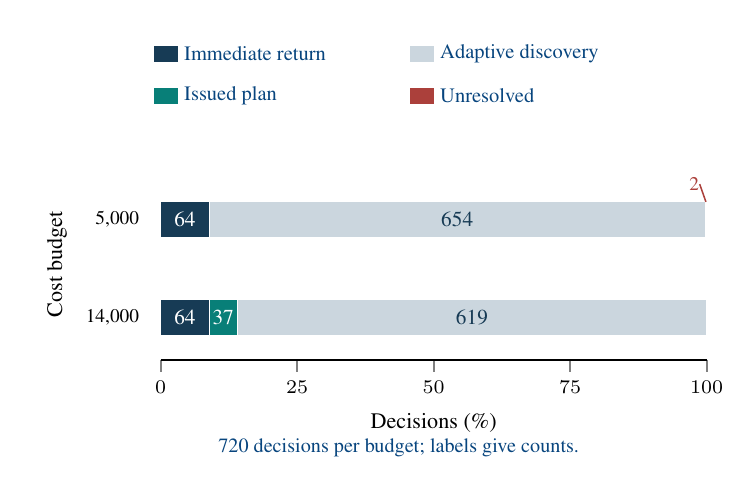
\begin{tikzpicture}[x=1in,y=1in]%
\path[use as bounding box] (0,0) rectangle (3.5,2.2);%
\begin{pgfinterruptboundingbox}%
\begin{axis}[jsc axis,at={(0.665in,0.539in)},anchor=south west,%
width=2.73in,height=0.957in,%
xmin=0,xmax=100,ymin=-.43,ymax=1.52,xtick={0,25,50,75,100},%
ytick={1,0},yticklabels={{5,000},{14,000}},ytick style={draw=none},%
y axis line style={draw=none},ylabel={Cost budget},xlabel={Decisions (\%)},%
]%
\path[fill=jscDark,draw=white,line width=.3pt] (axis cs:0,0.815) rectangle (axis cs:8.8888888888888893,1.185);%
\node[font=\jscfont{7.7},text=white,inner sep=0] at (axis cs:4.4444444444444446,1.0) {64};%
\path[fill=jscLight,draw=white,line width=.3pt] (axis cs:8.8888888888888893,0.815) rectangle (axis cs:99.722222222222214,1.185);%
\node[font=\jscfont{7.7},text=jscDark,inner sep=0] at (axis cs:54.305555555555557,1.0) {654};%
\path[fill=jscUnresolved,draw=white,line width=.3pt] (axis cs:99.722222222222214,0.815) rectangle (axis cs:99.999999999999986,1.185);%
\draw[jscUnresolved,line width=.55pt] (axis cs:99.8611111111111,1.18)--(axis cs:98.722222222222214,1.3599999999999999);%
\node[anchor=east,font=\jscfont{7},text=jscUnresolved,inner sep=0] at (axis cs:98.722222222222214,1.3599999999999999) {2};%
\path[fill=jscDark,draw=white,line width=.3pt] (axis cs:0,-0.185) rectangle (axis cs:8.8888888888888893,0.185);%
\node[font=\jscfont{7.7},text=white,inner sep=0] at (axis cs:4.4444444444444446,0.0) {64};%
\path[fill=jscTeal,draw=white,line width=.3pt] (axis cs:8.8888888888888893,-0.185) rectangle (axis cs:14.027777777777779,0.185);%
\node[font=\jscfont{7.7},text=white,inner sep=0] at (axis cs:11.458333333333334,0.0) {37};%
\path[fill=jscLight,draw=white,line width=.3pt] (axis cs:14.027777777777779,-0.185) rectangle (axis cs:100,0.185);%
\node[font=\jscfont{7.7},text=jscDark,inner sep=0] at (axis cs:57.013888888888893,0.0) {619};%
\end{axis}%
\path[fill=jscDark] (0.63,2.03) rectangle (0.75,2.11);%
\node[font={\jscfont{7.4}},text=jscNavy,anchor=west,align=center,inner sep=0pt] at (0.78,2.07) {Immediate return};%
\path[fill=jscLight] (1.9100000000000001,2.03) rectangle (2.0300000000000002,2.11);%
\node[font={\jscfont{7.4}},text=jscNavy,anchor=west,align=center,inner sep=0pt] at (2.06,2.07) {Adaptive discovery};%
\path[fill=jscTeal] (0.63,1.82) rectangle (0.75,1.9000000000000001);%
\node[font={\jscfont{7.4}},text=jscNavy,anchor=west,align=center,inner sep=0pt] at (0.78,1.86) {Issued plan};%
\path[fill=jscUnresolved] (1.9100000000000001,1.82) rectangle (2.0300000000000002,1.9000000000000001);%
\node[font={\jscfont{7.4}},text=jscNavy,anchor=west,align=center,inner sep=0pt] at (2.06,1.86) {Unresolved};%
\node[font={\jscfont{7.3}},text=jscNavy,anchor=center,align=center,inner sep=0pt] at (1.855,0.099) {720 decisions per budget; labels give counts.};%
\end{pgfinterruptboundingbox}%
\end{tikzpicture}%
\endgroup%
}
\caption{Observed outcomes of the sufficient-plan controller. Each budget
uses the same 720 tapes; time allowances are 4000 and 9000 units. All paths
include the 1152-unit audit. Successful issued plans are distinguished from
immediate verification and adaptive discovery.}
\label{fig:validity-outcomes}
\end{figure}
Of 1312 post-audit attempts, 37 issue plans; all discard history and complete under the larger budget, reserving/spending $11682.27/60.97$ additional units on average. Immediate/discovery correct counts are $128/1273$, with two unresolved. Matched fresh pilots reproduce every audited completion. Adaptive and sufficient excess costs are $9.42$ and $9.24$, with respective paired 95\% intervals $[-2.78,20.96]$ and $[-2.98,20.78]$: no net reuse benefit. A separate zero-shift reference's 160 historical completions assume stronger validity information.

\label{app:v37-study}
\emph{Guarded confirmation.} Nine methods use 21 declared labels, 32 tapes each, and two budgets (1344 attempts/method); three extension tuples duplicate originals on independent tapes. The primary fixes fresh acquisition actions and uses audited history only in verification/promises. Paired bootstraps preserve labels, tapes, and budgets. Declared targets are a saving lower endpoint above 2\% and completion-difference lower endpoint above $-1$ point.

\begin{table}[t]
\centering\small
\caption{Guarded confirmation: all 1344 decisions per method. Remaining decisions are unresolved; none is incorrect.}
\label{tab:v37-methods}
\begin{tabular}{@{}lrr@{}}
\toprule
Method&Mean cost&Correct\\
\midrule
Fresh proportional&3021.64&1128\\
Fresh repaired&2962.29&1128\\
Fresh slack&2947.11&1128\\
Guarded fresh&2996.73&1129\\
Audited, history-guided&2994.15&1128\\
Audited, balanced&3015.73&1129\\
Audited, fixed fresh actions&2992.60&1129\\
Earlier audited repaired&3130.14&1128\\
Earlier sufficient&3130.14&1128\\
\bottomrule
\end{tabular}
\end{table}
Primary saving is $.138\%$ (95\% interval $[.082,.201]\%$), below the 2\% target. Both primary and guarded fresh complete 575/576 original-grid and 554/768 extension decisions; 192 attempts are boundary/low-margin cases. Only 57 paths save strictly (maximum 304), all respecting fixed-action cost/duration ordering. Relative to fresh repaired, primary costs 1.023\% more for one extra completion. Its 4.394\% gain over earlier audited controllers changes initial auditing and does not isolate planning.
\begin{figure}[t]
\centering
\resizebox{\columnwidth}{!}{% Editable TikZ; coordinates are inches unless inside an axis.
% Numerical values come from data/; see data/PROVENANCE.json.
\begingroup%
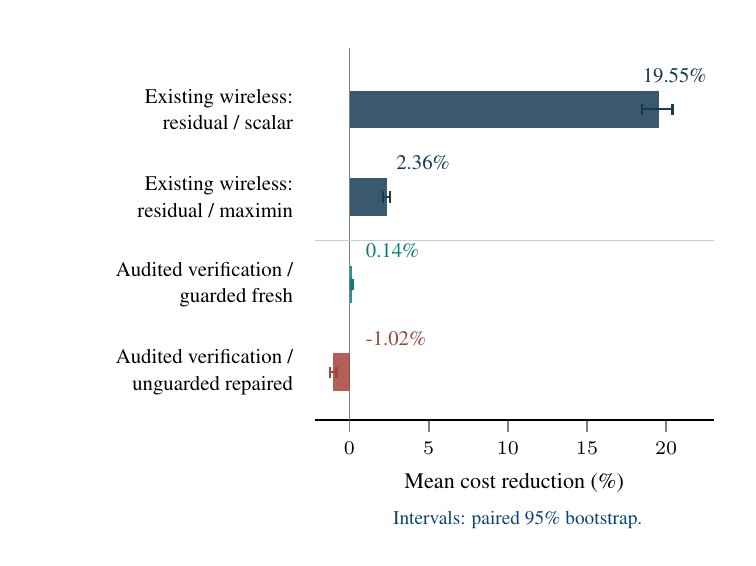
\begin{tikzpicture}[x=1in,y=1in]%
\path[use as bounding box] (0,0) rectangle (3.5,2.55);%
\begin{pgfinterruptboundingbox}%
\begin{axis}[jsc axis,at={(1.435in,0.5865in)},anchor=south west,%
width=1.995in,height=1.8615in,%
xmin=-2.2,xmax=23,ymin=-.55,ymax=3.7,xtick={0,5,10,15,20},ytick={3,2,1,0},%
yticklabels={{Existing wireless:\\residual / scalar},{Existing wireless:\\residual / maximin},%
{Audited verification /\\guarded fresh},{Audited verification /\\unguarded repaired}},%
yticklabel style={font=\jscfont{7.5},align=right},ytick style={draw=none},y axis line style={draw=none},%
xlabel={Mean cost reduction (\%)},%
]%
\draw[gray,line width=.65pt] (axis cs:0,-.55)--(axis cs:0,3.7);%
\draw[gray!40,line width=.5pt] (axis cs:-2.2,1.5)--(axis cs:23,1.5);%
\path[fill=jscDark,fill opacity=.85] (axis cs:0,2.785) rectangle (axis cs:19.550831216690224,3.215);%
\draw[jscDark,line width=.8pt] (axis cs:18.458995902889857,3.0)--(axis cs:20.396608603933906,3.0);%
\draw[jscDark,line width=.8pt] ([yshift=-2pt]axis cs:18.458995902889857,3.0)--([yshift=2pt]axis cs:18.458995902889857,3.0);%
\draw[jscDark,line width=.8pt] ([yshift=-2pt]axis cs:20.396608603933906,3.0)--([yshift=2pt]axis cs:20.396608603933906,3.0);%
\node[anchor=south east,font=\jscfont{7.5},text=jscDark,inner sep=0] at (axis cs:22.6,3.3) {19.55\%};%
\path[fill=jscDark,fill opacity=.85] (axis cs:0,1.785) rectangle (axis cs:2.3597073718749861,2.215);%
\draw[jscDark,line width=.8pt] (axis cs:2.1344010295820777,2.0)--(axis cs:2.571983988487665,2.0);%
\draw[jscDark,line width=.8pt] ([yshift=-2pt]axis cs:2.1344010295820777,2.0)--([yshift=2pt]axis cs:2.1344010295820777,2.0);%
\draw[jscDark,line width=.8pt] ([yshift=-2pt]axis cs:2.571983988487665,2.0)--([yshift=2pt]axis cs:2.571983988487665,2.0);%
\node[anchor=south west,font=\jscfont{7.5},text=jscDark,inner sep=0] at (axis cs:2.921983988487665,2.3) {2.36\%};%
\path[fill=jscTeal,fill opacity=.85] (axis cs:0,0.785) rectangle (axis cs:0.13784867185336,1.215);%
\draw[jscTeal,line width=.8pt] (axis cs:0.082286637516229999,1.0)--(axis cs:0.20054833344214001,1.0);%
\draw[jscTeal,line width=.8pt] ([yshift=-2pt]axis cs:0.082286637516229999,1.0)--([yshift=2pt]axis cs:0.082286637516229999,1.0);%
\draw[jscTeal,line width=.8pt] ([yshift=-2pt]axis cs:0.20054833344214001,1.0)--([yshift=2pt]axis cs:0.20054833344214001,1.0);%
\node[anchor=south west,font=\jscfont{7.5},text=jscTeal,inner sep=0] at (axis cs:1,1.3) {0.14\%};%
\path[fill=jscRed,fill opacity=.85] (axis cs:0,-0.215) rectangle (axis cs:-1.0233058850951799,0.215);%
\draw[jscRed,line width=.8pt] (axis cs:-1.2327670066285701,0.0)--(axis cs:-0.81512624104683995,0.0);%
\draw[jscRed,line width=.8pt] ([yshift=-2pt]axis cs:-1.2327670066285701,0.0)--([yshift=2pt]axis cs:-1.2327670066285701,0.0);%
\draw[jscRed,line width=.8pt] ([yshift=-2pt]axis cs:-0.81512624104683995,0.0)--([yshift=2pt]axis cs:-0.81512624104683995,0.0);%
\node[anchor=south west,font=\jscfont{7.5},text=jscRed,inner sep=0] at (axis cs:1,0.3) {-1.02\%};%
\end{axis}%
\node[font={\jscfont{7}},text=jscNavy,anchor=center,align=center,inner sep=0pt] at (2.45,0.08925) {Intervals: paired 95\% bootstrap.};%
\end{pgfinterruptboundingbox}%
\end{tikzpicture}%
\endgroup%
}
\caption{Separate frozen comparisons. The upper rows confirm existing nine-configuration wireless controllers on 32 complete four-goal sequences; the lower rows evaluate the new audited-verification variant on 1344 two-instrument decisions. Positive values denote lower all-attempt cost. The last comparison has one additional completion for the audited variant. Intervals preserve the paired experimental units; the populations and controller interfaces are not pooled.}
\label{fig:v37-costs}
\end{figure}
Primary/guarded fresh issue 500/484 promises, and all primary promises complete. Earlier sufficient acquisition issues 39/1152 under a different audit and $.105$ allowance. Primary mean spent/reserved-additional/actual-additional costs are $874.13/7352.62/347.89$; advertised/actual totals are $8226.76/1222.03$ (median ratio 6.75). Selected successes and unacquired endpoint replays establish no uniform conditional guarantee.
\begin{figure}[t]
\centering
\resizebox{\columnwidth}{!}{% Editable TikZ; coordinates are inches unless inside an axis.
% Numerical values come from data/; see data/PROVENANCE.json.
\begingroup%
\begin{tikzpicture}[x=1in,y=1in]%
\path[use as bounding box] (0,0) rectangle (3.5,3.05);%
\begin{pgfinterruptboundingbox}%
\begin{axis}[jsc axis,at={(0.63in,0.5795in)},anchor=south west,%
width=2.765in,height=2.1655in,%
xmode=log,ymode=log,xmin=8,xmax=16000,ymin=8,ymax=16000,%
xtick={10,100,1000,10000},ytick={10,100,1000,10000},%
xlabel={Actual additional cost},ylabel={Advertised additional cost},%
]%
\addplot[only marks,mark=*,mark size=1.5pt,mark options={draw opacity=0,fill=jscDark,fill opacity=.48}] table[x=actual,y=advertised,col sep=comma] {\jscDataPath/v37_promise_points_5000.csv};%
\addplot[only marks,mark=*,mark size=1.5pt,mark options={draw opacity=0,fill=jscTeal,fill opacity=.48}] table[x=actual,y=advertised,col sep=comma] {\jscDataPath/v37_promise_points_14000.csv};%
\addplot[gray,dashed,line width=.8pt] coordinates {(8,8) (16000,16000)};%
\node[anchor=south east,font=\jscfont{7},align=left,inner sep=0] at (rel axis cs:.95,.07)%
  {\textcolor{jscDark}{$\bullet$}\quad Budget 5,000\\%
   \textcolor{jscTeal}{$\bullet$}\quad Budget 14,000\\%
   \textcolor{gray}{\rule[2pt]{3pt}{.5pt}\,\rule[2pt]{3pt}{.5pt}}\quad Equal cost};%
\end{axis}%
\node[font={\jscfont{7.5}},text=jscNavy,anchor=west,align=center,inner sep=0pt] at (0.63,2.867) {500 issued promises};%
\end{pgfinterruptboundingbox}%
\end{tikzpicture}%
\endgroup%
}
\caption{Advertised and actual additional acquisition cost for the primary controller's 500 issued promises. Both axes are logarithmic. All promises complete in these trials, but reservations are conservative. These selected-promise diagnostics complement the all-attempt comparison in Table~\ref{tab:v37-methods}; they do not establish a conditional probability guarantee.}
\label{fig:v37-promises}
\end{figure}
Separate four-goal epochs share an evidence/cap ledger and risk $.03/4$ across thresholds $(5.8,4.8)\to(2.9,1.9)\to(1.4,.9)\to(5.8,4.8)$. Both primary/guarded fresh complete 563/576 epochs, costing $2196.56/2210.54$ (saving $.633\%$, interval $[.319,1.022]\%$). Primary can cost more at goal three; final relaxed goals need no reports. History-guided/balanced variants cost $2184.72/2379.14$ with 563/562 completions.

The separate nine-pair confirmation uses 32 new four-goal sequences/interface. Residual reaches estimated alternative distance $1.10\beta^2$ at minimum cost. Custom information-maximin maximizes minimum distance using an added-cost planning allowance of current-goal expenditure plus $\sum_ec_e$ (64 iterations, tolerance $.005$). This allowance is not a hard budget; the shared executor enforces original count/time limits, unlike resource-aware planning in the acquisition-design section of the theoretical supplement. Residual/scalar costs are $2661.84/3308.72$ (19.55\%, interval 18.46--20.40\%); residual/custom-maximin costs are $2739.90/2806.12$ (2.36\%, interval 2.13--2.57\%). All 512 decisions are correct; 22/32 intermediate and all loose requests need no reports. The development/final attempts, detailed audit records, and vendored comparison source cited by the original manuscript were not supplied. The two-instrument controller is not evaluated on nine pairs.

\section{System Boundaries and Evidence Scope}
\subsection{Instrumentation, Priors, and Agent Operation}
\label{app:operating-study}
The four-configuration model has $\theta=(r_0,r_1,w_{00},w_{01},w_{10},w_{11})$ and $D_{ij}=r_i+w_{ij}$, including nominal stage terms. Aggregate rank is 4, increasing to 5/6 with one/two radio counters. Charges are $(1.6,2.4,2.6,3.4)$, tolerance $.05$, and total/radio/server limits $24/3.8/8.5$ ms. Reports average 64 independent finite-buffer FCFS pre-admission workload draws, including rejected jobs: the target is diagnostic mean, not offered-job latency. Studies A--C start with 256 reports/aggregate (sunk 1920), batches 32, and caps 4096. Prefix radii are
$$h_e(n)=\sqrt{(2\sigma_e^2/n)\log(2\cdot6\cdot4096/\delta_{\rm on})}.$$
We intersect earlier intervals, priors, and admitted contrasts without resetting goal risk; empty intersections return model conflict. Exact-rational LP-witness audits check algebra separately from coverage.

\emph{A: common allocation.} Both verifiers use smallest-count acquisition, tied fast radio/slow radio/aggregates, truncated at full batches for deadlines 150/2000. Thirty-two seeds pair states shifted by $+2$ ms radio/$-2$ ms server, preserving aggregates/nonnegativity but changing the valid answer (configuration 3/infeasibility). Aggregate-only correct completion is at most $\delta$; nonabstention may reach $2\delta$. This construction changes server nominal terms, not merely the FCFS random seed.
\begin{table}[t]
\centering\small
\caption{Original zero-lower-bound comparison: correct count / mean new cost in each matched state at duration 2000. Completion counts also hold at 150.}
\label{tab:v41-capability}
\begin{tabular}{@{}lrr@{}}
\toprule
Access&Joint&Componentwise\\
\midrule
Aggregate only&0/32;2449.92&0/32;2449.92\\
Aggregate+fast radio&32/32;384&0/32;6745.92\\
All six&32/32;384&32/32;768\\
\bottomrule
\end{tabular}
\end{table}
Joint exclusion uses total delay above $3.8+8.5$ without identifying the violated stage; selected-action feasibility still needs stage evidence. At 150, unresolved aggregate-only/single-counter componentwise costs are $169.92/768$. Wilson 95\% intervals for 32/32 and 0/32 are $[89.3,100]/[0,10.7]\%$; two deadlines locate no transition.

\label{app:prior-sensitivity}
\emph{Prior correction.} The generator's valid radio minima $(3.88845,1.54168)$ ms were omitted originally. Replay strengthens these equally, retaining tapes, bands, and goals, and adds no invalid server bounds. Both verifiers then complete 32/32 at cost 384/duration 64 in each state: the one-counter advantage disappears. Below, original practical curves explicitly retain the broader zero-lower-bound prior. The full prior-sensitivity replay records were not supplied.

\emph{B: interactions.} Under radio-dependent server loading, flexible and calibrated-contrast models certify infeasibility from history in all 16 trials; nominal-equality modeling gives 16 conflicts. A constructed common server shift preserves contrasts. All 32 calibration sets cover, with no demonstrated acquisition-cost benefit or physical-transfer guarantee. The supplied text does not specify the separate calibration expenditure, risk split, or full interaction parameters.

\emph{C: common verifier.} Coverage/custom-maximin/residual share flexible priors, all instruments, 16 seeds/coupling, and duration 2000. Common LP repair produces regularized centers; plans cache at most 256 reports and maximin uses 12 iterations. At zero coupling all complete at costs $384/454.08/524.16$ and controller times $.038/.076/.143$ s. At $.24$, history completes all at zero new cost. Fixed batches give degenerate paired intervals, not population certainty. This adverse comparison is separate from nine-pair gains.

\emph{D: agent loop.} One language-model agent accesses public goals/evidence through proposal, acquisition, verification, and authorization tools. Isolation is procedural; the exact model version is unavailable. Loose/joint/loose goals share history; an announced change quarantines it before the final joint goal. Each epoch uses risk $.025$ and cost/duration caps 2000. Agent and deterministic coverage return $0,3,0$, then infeasibility. Their totals are 23/45 actions, costs $2133.76/2124.80$, and durations $729.44/735.20$; the agent acquires 448 reports, none at loose goals. One sequence proves no LLM advantage. The cited attempts, transcripts, 16 guard checks, and certificate/resource replay files were not supplied.

\begin{figure*}[t]
\centering
\resizebox{\textwidth}{!}{% Editable TikZ; coordinates are inches unless inside an axis.
% Numerical values come from data/; see data/PROVENANCE.json.
\begingroup%
\begin{tikzpicture}[x=1in,y=1in]%
\path[use as bounding box] (0,0) rectangle (8.08143888888889,3.388913194444444);%
\begin{pgfinterruptboundingbox}%
\begin{axis}[jsc axis,at={(0.57in,0.84in)},anchor=south west,%
width=3.48in,height=2.21in,%
xmin=0,xmax=512,ymin=0,ymax=1.02,xtick={0,100,200,300,400,500},ytick={0,.2,.4,.6,.8,1},title={Accurate server counter},%
axis lines=box,axis line style={line width=.7pt},major grid style={gray!18},grid=major,tick label style={font=\jscfont{8}},%
xlabel={Modeled acquisition deadline},xlabel style={font=\jscfont{9}},title style={font=\jscfont{10}},%
ylabel={Correct-completion limit},ylabel style={font=\jscfont{9}},%
]%
\addplot[gray,line width=1.6pt,dashed] table[x=deadline,y=correct,col sep=comma] {\jscDataPath/frontier_accurate_server_aggregate.csv};%
\addplot[jscRadio,line width=1.6pt] table[x=deadline,y=correct,col sep=comma] {\jscDataPath/frontier_accurate_server_radio.csv};%
\addplot[jscServer,line width=1.6pt] table[x=deadline,y=correct,col sep=comma] {\jscDataPath/frontier_accurate_server_server.csv};%
\addplot[jscBoth,line width=1.6pt,dashed] table[x=deadline,y=correct,col sep=comma] {\jscDataPath/frontier_accurate_server_both.csv};%
\addplot[black,dotted,line width=.8pt] coordinates {(0,.95) (512,.95)};%
\end{axis}%
\begin{axis}[jsc axis,at={(4.45in,0.84in)},anchor=south west,%
width=3.48in,height=2.21in,%
xmin=0,xmax=512,ymin=0,ymax=1.02,xtick={0,100,200,300,400,500},ytick={0,.2,.4,.6,.8,1},title={Accurate radio counter},%
axis lines=box,axis line style={line width=.7pt},major grid style={gray!18},grid=major,tick label style={font=\jscfont{8}},%
xlabel={Modeled acquisition deadline},xlabel style={font=\jscfont{9}},title style={font=\jscfont{10}},%
yticklabels=\empty,%
]%
\addplot[gray,line width=1.6pt,dashed] table[x=deadline,y=correct,col sep=comma] {\jscDataPath/frontier_accurate_radio_aggregate.csv};%
\addplot[jscRadio,line width=1.6pt] table[x=deadline,y=correct,col sep=comma] {\jscDataPath/frontier_accurate_radio_radio.csv};%
\addplot[jscServer,line width=1.6pt] table[x=deadline,y=correct,col sep=comma] {\jscDataPath/frontier_accurate_radio_server.csv};%
\addplot[jscBoth,line width=1.6pt,dashed] table[x=deadline,y=correct,col sep=comma] {\jscDataPath/frontier_accurate_radio_both.csv};%
\addplot[black,dotted,line width=.8pt] coordinates {(0,.95) (512,.95)};%
\end{axis}%
\draw[gray,line width=1pt,dashed] (0.67,.20)--(0.91,.20);%
\node[font={\jscfont{8}},text=jscNavy,anchor=west,align=center,inner sep=0pt] at (0.97,0.2) {Aggregate only};%
\draw[jscRadio,line width=1pt] (2.1,.20)--(2.34,.20);%
\node[font={\jscfont{8}},text=jscNavy,anchor=west,align=center,inner sep=0pt] at (2.4,0.2) {Radio counter};%
\draw[jscServer,line width=1pt] (3.62,.20)--(3.8600000000000003,.20);%
\node[font={\jscfont{8}},text=jscNavy,anchor=west,align=center,inner sep=0pt] at (3.92,0.2) {Server counter};%
\draw[jscBoth,line width=1pt,dashed] (5.18,.20)--(5.42,.20);%
\node[font={\jscfont{8}},text=jscNavy,anchor=west,align=center,inner sep=0pt] at (5.4799999999999995,0.2) {Both counters};%
\draw[black,line width=1pt,dotted] (6.7,.20)--(6.94,.20);%
\node[font={\jscfont{8}},text=jscNavy,anchor=west,align=center,inner sep=0pt] at (7.0,0.2) {95\% target};%
\end{pgfinterruptboundingbox}%
\end{tikzpicture}%
\endgroup%
}
\caption{Exact correct-completion limits at absolute stage margin $0.2$,
wrong-return risk $0.05$, and hard cost cap 512. Lines give the exact
reference. Counter precision changes
which instrumentation can meet a deadline. The aggregate-only line is a
randomized 5\% upper bound; our operational policies always abstain in
that case. Radio and both-counter curves coincide in the right panel.
Durations are modeled acquisition units.}
\label{fig:v42-scalar-frontier}
\end{figure*}

\begin{table*}[t]
\centering\small
\caption{Practical results at deadline 512. Ordered pairs correspond to radio limits $(3.1,3.8)$ ms; each correct count is out of 16 seeds. C: coverage; G: goal-directed. Both orientations agree with all probes. Costs include unresolved attempts; unequal completion prevents equivalent-service cost ratios. History adds 1920 sunk units.}
\label{tab:v42-practical}
\begin{tabular}{@{}cclrrrr@{}}
\toprule
Orientation&History/probe&Access&C correct&G correct&C cost&G cost\\
\midrule
Both&0&All&(0, 0)&(16, 16)&(1615.10, 1615.10)&(1628.75, 1004.89)\\
Both&256&All&(15, 16)&(16, 16)&(2517.00, 564.00)&(1275.00, 297.00)\\
0&0&Fixed 5&(0, 0)&(16, 16)&(1248.00, 1248.00)&(1564.69, 974.63)\\
0&256&Fixed 5&(16, 16)&(16, 16)&(1275.00, 297.00)&(1275.00, 297.00)\\
1&0&Fixed 5&(0, 0)&(0, 0)&(1248.00, 1248.00)&(880.04, 918.77)\\
1&256&Fixed 5&(0, 0)&(0, 0)&(3072.00, 3072.00)&(832.20, 832.20)\\
\bottomrule
\end{tabular}
\end{table*}

\subsection{Completion Frontiers and Practical Curves}
\label{app:deadline-study}
The scalar Gaussian benchmark has cheap-stage means $(6+\vartheta,6-\vartheta)$, limits $(6,7,13)$, and a costlier safe backup. For $0<|\vartheta|<.8$, negative/positive margins uniquely favor cheap/backup. Centered aggregate/radio/server means are $0,\vartheta,-\vartheta$. Radio/server costs are $(1,6)$, durations $(1,4)$, and accurate-server variances $(1,1/9)$, reversed for accurate radio; history is empty and cost/count caps are 512. A public-parameter dynamic program maximizes precision $A_{\max}(H)$ for integer $H\leq512$. Theorem~\ref{thm:scalar-deadline} gives the exact frontier and attaining endpoint test. At zero precision, operational policies abstain although randomization permits 5\% correct completion.
\begin{table}[t]
\centering\small
\caption{Exact first modeled deadline for 95\% correct completion, wrong-return risk $.05$, and cost cap 512. Dashes remain unattainable with more time. Both signs agree.}
\label{tab:v42-targets}
\begin{tabular}{@{}llrrr@{}}
\toprule
Catalogue&Counter&$|\vartheta|=.1$&$.2$&$.4$\\
\midrule
Accurate server&Radio&---&271&68\\
&Server&---&124&32\\
&Both&---&121&32\\
Accurate radio&Radio&121&31&8\\
&Server&---&---&272\\
&Both&121&31&8\\
\bottomrule
\end{tabular}
\end{table}


At margin $.1$, accurate-server precision caps at 767 and completion at $.869626$. Sequential execution orders the same design by precision/duration, spending one-sided risk $.01/[j(j+1)]$ at report $j<N$ and $.04$ at the endpoint (single-report risk $.05$). Each deadline defines a separate valid policy.

Evaluation crosses margins $\pm.1,\pm.2,\pm.4$ and deadlines $0,8,32,128,512$: 4096 seeds in each of 480 cells, totaling 1,966,080 correlated outcomes. Maximum endpoint discrepancy across 144 positive-information cells is 1.545 points (standardized 2.628). At preselected $\vartheta=.2$, both counters/accurate server/$H=128$, endpoint versus sequential returns 3919/3877 correct, 0/2 wrong, and 177/217 unresolved, costing $192/164.883$. Other endpoints also trade lower cost for missed or incorrect returns; complete outcome records were not supplied. Early stopping does not improve cost and completion uniformly.

\emph{Practical policies.} The bounded six-mean/zero-lower-bound model crosses both radio-row orientations, radio limits 3.8/3.1, history 0/256, and all probes versus aggregates plus fixed counter 5. The counter is useful in only one orientation. Caps/risk/batches are $4096/.05/4$; history costs 1920. Coverage selects smallest absolute count with seeded random tie order. Goal-directed acquisition targets the cheapest unexcluded configuration and maximizes unresolved directional uncertainty reduction/duration; regularization guides allocation only. One sequence/policy is truncated before unaffordable batches at $H=0,16,32,64,128,256,512$. Sixteen paired seeds yield 512 traces/3584 deadline views; Wilson and 10000 seed-cluster bootstrap intervals preserve paired orientations/deadlines. These curves are policy-specific.

The wrong-counter obstruction $v=(0,2,0,0,-2,-2)$ preserves aggregate and observed slow-radio laws but changes configuration 3 to infeasibility, respecting the stated prior/noise model. Correct completion is therefore at most $\delta$ for every deadline; known server-row equality removes that alternative. Unresolved all-instrument prefixes prove no such impossibility. The original source references additional protocols and design/tape/stopping/certificate audits that were not supplied. The 604 approved deadline views contain no error but are correlated.

\subsection{Physical Evidence and Reproduction Limits}
\label{app:deployment-protocol}
No experiment uses a live wireless--edge link. Additive-model holdout RMSE rises from $.166$ ms under shared load to $2.066/4.449$ ms with server interactions (noiseless $2.047/4.386$): sampling cannot remove structural error. Historical EdgeDroid~\cite{edgedroid2019} and localhost summaries lack the raw observations, harnesses, splits, or timestamp logs needed for reproduction. Missing latencies are not imputed; observed residuals do not validate unseen stage delays.

The original manuscript reports 18 synthetic integrity cases that verify only the record schema; their source files were not supplied.


\section{Simulation-Based Continuation Selection}
The following construction preserves the full simulation-based selector guarantee from the original supplementary source. Probe $e$ has Gaussian mean $a_e^\T\theta$, variance $\sigma_e^2$, and one-report information matrix $G_e=a_ea_e^\T/\sigma_e^2$. The set $\mathcal Q_{\rm int}$ denotes the original legal integer fresh-count vectors under the total count, time, and cost caps; discovery counts remain charged. For $M\succeq0$, write $\|v\|_M^2=v^\T Mv$, and use $P^\dagger$ for the Moore--Penrose inverse. The common verifier has a simultaneous unconditional wrong-return risk at most $\delta$ under every admissible acquisition rule. The notation $P^\star(\delta,B)$ denotes the paper's unrestricted correct-completion frontier under this risk and resource bound. These are the assumptions under which the construction below applies.

\subsection{An Implementable Continuation Guarantee}
\label{app:continuation-construction}
\label{app:v23selector}

At a legal discovery stopping time, let $\mathcal H$ contain retained/discovery reports and $d$ the discovery counts. Completed returns are absorbing; otherwise $K_c$ executable candidates $\pi_k(\mathcal H)$ share the original verifier and remaining set $\mathcal Q_{\mathcal H}=\{n\in\mathbb Z_+^E:d+n\in\mathcal Q_{\rm int}\}$. The fixed-goal Gaussian subclass has a unique answer at every admitted regular coefficient.

Choose a center $\vartheta_0=\widetilde\theta(\mathcal H)$ and an anytime set $\mathcal C(\mathcal H)$ of coverage $1-\delta_{\rm est}$. For a set $\mathcal Q_{\mathcal H,k}$ containing all possible candidate counts, put
$$\rho_k=\sup_{v\in\mathcal C(\mathcal H)}
\max_{n\in\mathcal Q_{\mathcal H,k}}
\|v-\vartheta_0\|_{M_{\rm new}(n)},\qquad
M_{\rm new}(n)=\sum_e n_eG_e.$$
For $\mathcal C=\{v:\|v-\vartheta_0\|_P^2\leq2b\}$, $P\succeq0$, $b>0$, and componentwise quotas $n_k$, a valid radius is $\rho_k^2=2b\lambda_{\max}(P^{\dagger/2}M_{\rm new}(n_k)P^{\dagger/2})$ when $\range(M_{\rm new}(n_k))\subseteq\range(P)$; otherwise use infinity.

Let $q_v^k$ be the conditional probability of any verified return when future reports use coefficient $v$, holding actual history fixed. Prespecify candidates and $L_{\rm MC}$ independent simulations per candidate under $\vartheta_0$. Simultaneous conditional $1-\delta_{\rm MC}$ intervals $[l_k^{\rm MC},u_k^{\rm MC}]$ follow from Hoeffding half-width $\sqrt{\log(2K_c/\delta_{\rm MC})/(2L_{\rm MC})}$, or Clopper--Pearson tails $\delta_{\rm MC}/(2K_c)$. Candidates may share randomness. Define $T_\pm(q,r)=\Phi(\Phi^{-1}(q)\pm r)$, with continuous endpoints, and
\begin{equation}
L_k=T_-(l_k^{\rm MC},\rho_k),\qquad
U_k=T_+(u_k^{\rm MC},\rho_k).
\label{eq:v23transport}
\end{equation}
Use $[0,1]$ if $\rho_k=\infty$. Execute a maximizer $\widehat k$ of $L_k$ and put $\Delta=\max_kU_k-L_{\widehat k}$; an approximate selector uses its actual lower bound.

\begin{theorem}[Finite-confidence continuation intervals]
\label{thm:v23selector}
With probability at least $1-\delta_{\rm est}-\delta_{\rm MC}$ over
history, discovery, and simulation randomness, simultaneously
$$
 L_k\leq q_\theta^k\leq U_k\quad\text{for all }k,\qquad
 \max_k q_\theta^k-q_\theta^{\widehat k}\leq\Delta.
$$
The composed controller is uniformly $\delta$-safe. For conditional
correct-completion probabilities $p_\theta^k(\mathcal H)$, define the
same-discovery oracle for discovery strategy $D$,
$P^*_{D,K_c}(\theta)=\mathbb E_\theta\max_k p_\theta^k(\mathcal H)$.
Then
\begin{equation}
 \begin{split}
 \Pr_\theta\{\mathrm{correct\ return}\}
 &\geq\mathbb E_\theta L_{\widehat k}-\delta_{\rm est}-\delta_{\rm MC}-\delta,\\
 \Pr_\theta\{\mathrm{correct\ return}\}
 &\geq P^*_{D,K_c}(\theta)-\mathbb E_\theta\Delta\\
 &\quad-\delta_{\rm est}-\delta_{\rm MC}-\delta.
 \end{split}
 \label{eq:v23classguarantee}
\end{equation}
\end{theorem}

\begin{IEEEproof}
Condition on $\mathcal H,k$. On $\theta\in\mathcal C(\mathcal H)$, every continuation has Gaussian information separating $\theta,\vartheta_0$ at most $\rho_k^2$. The Gaussian information-time comparison proved in the associated paper and Neyman--Pearson applied to return and its complement give
$$T_-(q_{\vartheta_0}^k,\rho_k)\leq q_\theta^k
\leq T_+(q_{\vartheta_0}^k,\rho_k).$$
Actual history stays fixed; the selected center is not assigned a fixed Gaussian law. Combine monotonicity with simultaneous simulation coverage, then subtract endpoints for $\Delta$. No independence between confidence events is required.

Conditional on history and selection randomness, physical future reports are independent of simulations, so the composed return probability is $\mathbb E_\theta q_\theta^{\widehat k}$. Integrating the interval/gap bounds costs at most $\delta_{\rm est}+\delta_{\rm MC}$. Since $q_\theta^k\geq p_\theta^k$, subtract the common verifier's unconditional wrong-return risk $\delta$ once to obtain \eqref{eq:v23classguarantee}. Discovery returns remain absorbing.
\end{IEEEproof}

The guarantee provides neither conditional safety after selected history nor an impossibility test when $L_k$ is small. Larger quotas may enlarge $\rho_k$. Selection costs $O(K_cL_{\rm MC}NT_{\rm pl})$ for at most $N$ simulated reports and per-report computation $T_{\rm pl}$; charge this when the deadline includes computation.

Comparison to unrestricted $P^\star$ additionally subtracts the restriction gap
$$G_{D,K_c,\mathcal V}(\theta)=P^\star(\delta,B)-P^*_{D,K_c}(\theta)\geq0.$$
The finite-class oracle shares discovery, resources, and verifier, with $\theta$ a pointwise design constant, not implemented input. Hard budget $B$ makes its mean-cost cap redundant; a smaller expected-cost ceiling requires a separate feasibility certificate. The experiments do not bound this restriction gap. The optional quota-selection variants referenced by the original source were not supplied.


\subsection{Numerical Adaptive-Instrument Reference}
The separate finite-resource adaptive-separation example uses a near stage with absolute margin between $d_{\min}$ and $d_{\max}$ and another stage in $[-D_{\max},-D]$. Historical observations have fixed stage sums and do not reveal the relevant branch. We retain the full numerical specification:
$$
(d_{\min},d_{\max},D,D_{\max})=(0.1,0.25,1,2),\qquad
(\sigma_D^2,\sigma_1^2,\sigma_2^2)=(25,1,1).
$$
Coarse reports measure both stages, while a fine report measures its selected stage. Their durations are $(1,4,4)$, prices are $(1,8,8)$, and report caps are $(300,400,400)$. We use $(\delta,\delta_D,\delta_C)=(0.05,0.01,0.04)$, deadline $H=1500$, and budget $B=3000$. The adaptive rule takes 224 coarse reports, selects the larger coarse mean, and acquires 307 fine reports of that stage. Its duration is $224+4\cdot307=1452$ and its cost is $224+8\cdot307=2680$. The fixed-plan lower bounds in the theoretical supplement, including randomized plans, are $2164.43$ duration units and $4328.87$ cost units. This is the stated Gaussian numerical specialization under a separated-branch promise, not a replay of a physical deployment or evidence of general adaptive optimality.


\begin{thebibliography}{9}
\bibitem{lindner2022}
D. Lindner, S. Tschiatschek, K. Hofmann, and A. Krause, ``Interactively learning preference constraints in linear bandits,'' in \emph{Proc. ICML}, ser. PMLR, vol. 162, 2022, pp. 13505--13527.
\bibitem{edgedroid2019}
M. O. J. Olgu\'{i}n Mu\~noz, J. Wang, M. Satyanarayanan, and J. Gross, ``EdgeDroid: An experimental approach to benchmarking human-in-the-loop applications,'' in \emph{Proc. ACM HotMobile}, 2019, doi: 10.1145/3301293.3302353.
\end{thebibliography}
\end{document}
